\documentclass{beamer}

%!TEX root = ../main.tex
\usepackage[utf8]{inputenc}

\usepackage{lmodern}
\usepackage{booktabs}
\usepackage{graphicx}
\usepackage{listings}
%!TEX root = ../main.tex
\usetheme{Warsaw}
%\setbeamertemplate{footline}[frame number]


\title[Variáveis Determinantes - CPC e Enade]{Variáveis determinantes para formação do conceito preliminar de curso nas avaliações do Enade.}
\author[Guilherme]{Guilherme Souza}
\institute{Universidade Federal Fluminense}
\date{Niterói. \today}

%Boa tarde.
%Meu nome é Guilherme.
%Gostaria primeiramente de agradecer ao meu orientador Ariel, pela paciência e ter dedicado seu tempo em me orientar. 
%Queria agradecer aos senhores Professor Joel e Camilo por terem aceitado o convite de participar da banca do meu TCC.
%Bom mãos à obra...
%%%%%%%%%%%%%%%%%%%%%%%%%%%%%%%%%%%%%%
%Eu vou falar aqui hoje sobre avaliação do ensino, mais especificamente sobre as avaliações do Enade e o conceito preliminar de curso ou CPC
%Esse é o tema do meu TCC

\begin{document}
\begin{frame}
\titlepage
\end{frame}

%Importante citar os problemas que motivaram a pesquisa.
\begin{frame}{Problemas}
	Principais fatores que motivam a pesquisa:
	\begin{enumerate}
	%Percebe-se que, especificamente no caso brasileiro, o tema educação vem recebendo cada vez mais atenção governamental em termos de alocação de recursos. De acordo com Mendes (2015, p. 1), esta área passou a absorver parcelas significativas de destinações orçamentárias, sobretudo na última década. De acordo com o autor, estas receitas passaram de 4% em 2004 para 9,3% em 2014, um acréscimo de 130% no período. Isso revela uma importante transição da política educacional no país. Além disso, educação de uma forma geral é um tema importante por que ela trás vários benefícios agregados para a sociedade, como diminuição da pobreza e melhora até mesmo a saúde do indivíduo.
	\item Importância da qualificação superior para o país.
	%Como foi possível verificar pela revisão da literatura, a maioria dos estudos estão voltados a avaliar o ensino fundamental e médio. Existem poucos trabalhos direcionados a avaliar a qualidade da educação superior.
	\item Existem poucos estudos relacionando exames de desempenho e qualidade de cursos superiores.
	% Historicamente no Brasil há uma concentração maior do ensino superior nas instituições de ensino públicas (BARBOSA; FREIRE; CRISÓSTOMO, 2011), realidade que pode estar relacionada à inexistência de pagamento de mensalidades pelos alunos e a proliferação de instituições particulares com cursos de baixa qualidade. Isso gera necessidade ao governo de prestar atenção especial às políticas de ampliação de acesso ao ensino superior bem como criar mecanismos de avaliação, auditoria e gestão das IES de maneira geral. 
	\item Aumento significativo do número de instituições e cursos de baixa qualidade.
	%A prática de ranqueamento de instituições com base em pontuação no Enade parece ser uma prática comum, principalmente nos mecanismos de marketing de instituições de ensino particulares. De fato, isso é algo que se encontra presente desde que o INEP iniciou os ciclos de avaliação (VERHINE; DANTAS; SOARES, 2006, p. 294). Existe um grande gosto popular por tais comparações com base em disputa por posições, embora de nada sirvam para mensurar a capacidade de agregação de habilidades e competências dos estudantes nos cursos. (BRITO; REGINA, 2008, p. 847).
	\item Ranqueamento de cursos com base na nota do Enade deturpam os reais propósitos da formação superior.
	%Com a expansão da oferta, foram aprimorados mecanismos de mensuração da qualidade dos cursos prestados por instituições de ensino superior (IES) publicas e privadas. Com isso, é natural que a análise do desempenho e da qualidade do ensino superior tenha se tornado uma importante área de pesquisas com a utilização diversas metodologias quantitativas e qualitativas. Isso decorre da necessidade de mensurar a eficiência do gasto público em educação, principalmente por intermédio de indicadores, como a proporção de alunos por professor e o custo por estudante, por exemplo (COSTA et al., 2012, p. 417).
	\item Os indicadores de desempenho de cursos e instituições se tornaram interfaces para mensuração do gasto público.
	\end{enumerate}
\end{frame}

%Baseado nesse problemas eu formulei algumas perguntas:
\begin{frame}{Perguntas da Pesquisa}
	\begin{enumerate}
	%Determinar a qualidade de um produto acabado ou serviço de uma empresa é uma tarefa bem objetiva porque tem-se em mãos uma entrada e uma saída. A tarefa é verificar se aquela saída está de acordo com os padrões de fabricação e limites de custo, e pronto.
	%A avaliação da qualidade de cursos superiores ou instituições de ensino é bem mais difícil, porque você tem uma diversidade de dimensões passíveis de serem avaliadas. Além disso, as entradas e saídas nunca são as mesmas pois cada aluno tem um background diferente em termos de situação socio-economica e conhecimento prévio. Outro fator  que complica a mensuração da qualidade é a variedade de atores envolvidos e interesses. De forma ilustrativa, o gestor de recursos públicos poderia voltar sua atenção ao custo por aluno. O estudante, por outro lado, poderá valorizar mais a empregabilidade após formado – dimensão esta quase sempre negligenciada pelo primeiro observador. O professor universitário, por sua vez, poderia voltar sua preocupação a quantidade de alunos em sala de aula ou mesmo às condições de estabilidade.
	\item Como mensurar o desempenho de um curso de graduação?
	%Uma outra pergunta que é se o CPC, que é um indicador de desempenho dos cursos superiores originado pelo Enade, pode ser um parâmetro para determinar se um curso superior tem qualidade. 
	\item O Conceito Preliminar de Curso (CPC) do Enade é representativo da qualidade do curso?
	%O CPC é uma variável de resposta que é formada a partir de um conjunto de outras variáveis preditoras. Se eu posso afirmar que p CPC é capaz de mensurar a qualidade do curso de graduação eu posso verificar quais as variáveis desse conjunto de preditoras que mais participam. Com isso, eu posso informar o que deve ser feito em termos de investimentos para melhorar a qualidade desses cursos.
	\item Quais são as principais variáveis na composição do CPC?
	\end{enumerate}
\end{frame}

\begin{frame}{Metodologia}
	A pesquisa é qualitativa e quantitativa. Foram aplicadas as seguintes técnica:
	%Essa pesquisa é qualitativa e quantitativa. Qualitativa porque nela há uma tentativa de apresentar um entendimento sobre a metodologia de qualificação dos cursos por meio da análise da literatura disponível. É também quantitativa porque nela eu tento explicar as variáveis trabalhadas pelo Enade e o relacionamento entre elas com a aplicação na AED, ACP e da AF.
	\begin{enumerate}
		\item Análise Exploratória de dados
		%conhecer o conjunto de dados através de sua descrição com elementos visuais, como histogramas e tabelas; identificar os atributos de cada variável.
		\item Análise dos Componentes Principais
		%Reduzir um conjunto grande de variáveis em componentes capazes de explicar um evento pela concentração da variabilidade nos mesmos.
		% Procurou-se extrair perfis de variáveis representativas dos cursos superiores capazes de descrevê-los em arranjos significativos de fácil compreensão.
		\item Análise dos Fatores 
		%outra técnica de redução de dimensão utilizada para descrever variabilidade em um conjunto grande de variáveis correlacionadas com base em um número menor de variáveis não observadas (fatores).
	\end{enumerate}
\end{frame}

\begin{frame}{Ferramenta: R} 
	%Tem uma série de pontos fortes em relação ao R: a facilidade e velocidade de criação de visualização de dados, a capacidade de trabalhar com um número de dados muito superior ao do excel, uma vez que o R é limitado à capacidade de memória a processamento da máquina.
	%$R$ é uma linguagem e um ambiente para computação estatística e criação de gráficos similar a linguagem S desenvolvida pelo Bell Labs. É uma aplicação livre e de código aberto sob a licença GNU/GPL (General Public License)composta por uma extensa variedade de pacotes utilizados para as mais diferentes finalidades. O R é mantido por uma comunidade global de desenvolvedores e possui uma expressiva aceitação em pesquisas.
	\begin{enumerate}
	\item A linguagem
	\item Software livre
	\item Facilidades e capacidades

	\end{enumerate}
\end{frame}

\begin{frame}{Fluxo de Trabalho}
	%Essa é uma representação de como se deu o fluxo de trabalho. Os dados usados na pesquisa são públicos e disponíveis online. Esses dados foram obtidos e alimentados no R. 
	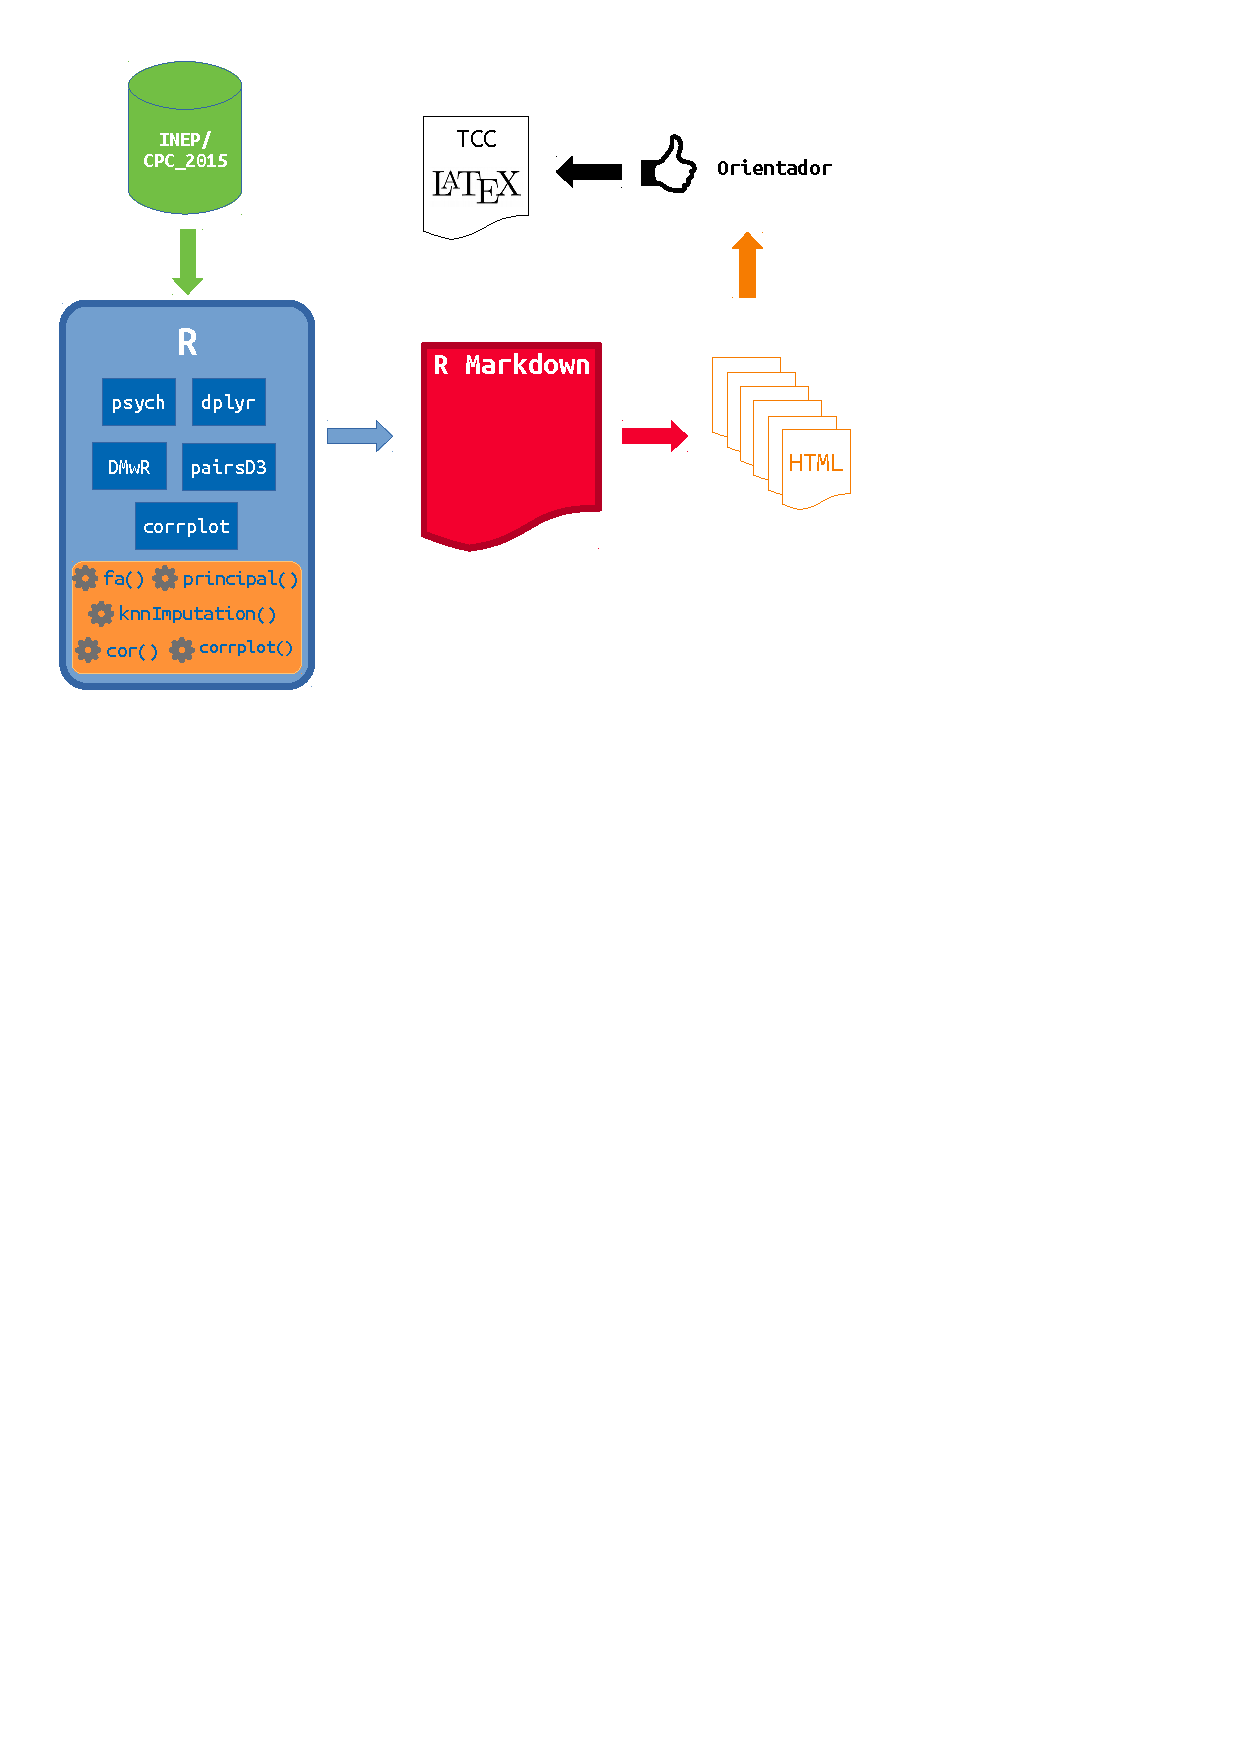
\includegraphics[width=1.1\textwidth]{images/work-flow}
\end{frame}

\section{Análise Exploratória de Dados}
	\begin{frame}{Informações sobre o censo}
		\begin{enumerate}
			\item Cursos avaliados:  8121
			\item IES's avaliadas:  1758
			\item Municípios com cursos avaliados:  753
			\item Estados com cursos avaliados:  27
			\item Percentual de participação nas provas:  81.4\%
		\end{enumerate}
	\end{frame}

	\begin{frame}{Cursos por região}
		% Please add the following required packages to your document preamble:
% \usepackage{booktabs}
% \usepackage{graphicx}
\begin{table}[H]
\centering
\resizebox{\textwidth}{!}{%
\begin{tabular}{@{}lllllll@{}}
\toprule
\textbf{Área de Enquadramento}           & \textbf{Centro Oeste} & \textbf{Nordeste} & \textbf{Norte} & \textbf{Sudeste} & \textbf{Sul} & \textbf{Total} \\ \midrule
ADMINISTRAÇÃO                            & 189                   & 312               & 97             & 841              & 367          & 1806           \\
DIREITO                                  & 117                   & 208               & 70             & 455              & 216          & 1066           \\
CIÊNCIAS CONTÁBEIS                       & 115                   & 190               & 71             & 444              & 224          & 1044           \\
TECNOLOGIA EM GESTÃO DE RECURSOS HUMANOS & 41                    & 69                & 17             & 314              & 82           & 523            \\
PSICOLOGIA                               & 39                    & 85                & 31             & 200              & 111          & 466            \\
PUBLICIDADE E PROPAGANDA                 & 30                    & 49                & 16             & 200              & 60           & 355            \\
TECNOLOGIA EM LOGÍSTICA                  & 15                    & 44                & 12             & 210              & 56           & 337            \\
JORNALISMO                               & 23                    & 49                & 22             & 126              & 55           & 275            \\
TECNOLOGIA EM MARKETING                  & 10                    & 37                & 7              & 167              & 50           & 271            \\
TECNOLOGIA EM GESTÃO FINANCEIRA          & 11                    & 23                & 5              & 139              & 45           & 223            \\
TECNOLOGIA EM PROCESSOS GERENCIAIS       & 9                     & 24                & 7              & 113              & 63           & 216            \\
CIÊNCIAS ECONÔMICAS                      & 15                    & 36                & 9              & 83               & 48           & 191            \\
DESIGN                                   & 8                     & 20                & 5              & 70               & 75           & 178            \\
TECNOLOGIA EM GESTÃO COMERCIAL           & 9                     & 32                & 6              & 77               & 46           & 170            \\
TURISMO                                  & 16                    & 35                & 10             & 61               & 27           & 149            \\
TECNOLOGIA EM GASTRONOMIA                & 10                    & 24                & 2              & 49               & 22           & 107            \\
RELAÇÕES INTERNACIONAIS                  & 9                     & 8                 & 5              & 58               & 21           & 101            \\
TEOLOGIA                                 & 8                     & 14                & 5              & 37               & 30           & 94             \\
TECNOLOGIA EM DESIGN DE INTERIORES       & 8                     & 14                & 2              & 38               & 20           & 82             \\
TECNOLOGIA EM GESTÃO DA QUALIDADE        & 6                     & 6                 & 48             & 15               & 6            & 81             \\
TECNOLOGIA EM COMÉRCIO EXTERIOR          & 2                     & 3                 & 2              & 57               & 16           & 80             \\
TECNOLOGIA EM DESIGN GRÁFICO             & 6                     & 12                & 4              & 43               & 12           & 77             \\
TECNOLOGIA EM GESTÃO PÚBLICA             & 15                    & 11                & 4              & 19               & 16           & 65             \\
SECRETARIADO EXECUTIVO                   & 7                     & 10                & 4              & 22               & 18           & 61             \\
TECNOLOGIA EM DESIGN DE MODA             & 2                     & 13                & 2              & 22               & 19           & 58             \\
ADMINISTRAÇÃO PÚBLICA                    & 6                     & 16                & 2              & 19               & 8            & 51             \\ \bottomrule
\end{tabular}%
}
\caption{Cursos por região}
\label{my-label}
\end{table}
	\end{frame}

	\begin{frame}{Percentual de cursos por Organização Acadêmica}
		\begin{figure}[H]
			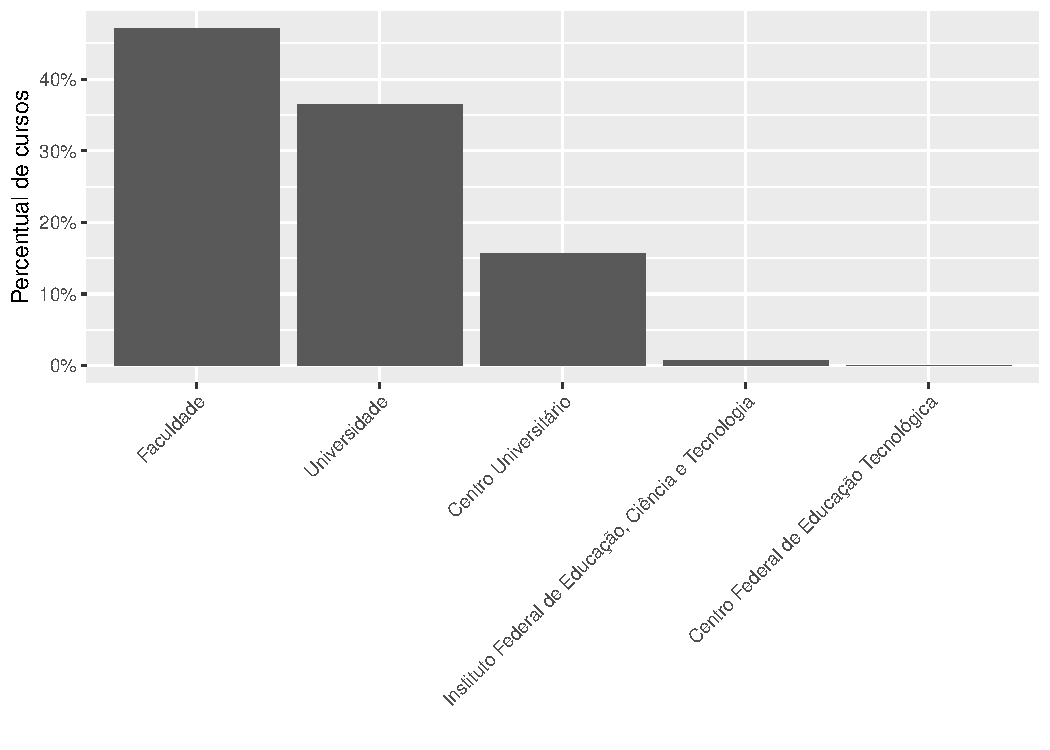
\includegraphics[scale=.50]{../graficos/latex-graph-percent-de-cursos-p-org-acad.pdf}
		\end{figure}
	\end{frame}

	\begin{frame}{Cursos com conceito}
		\begin{columns}
			\begin{column}{0.5\textwidth}
			   	 	\begin{figure}[H]
					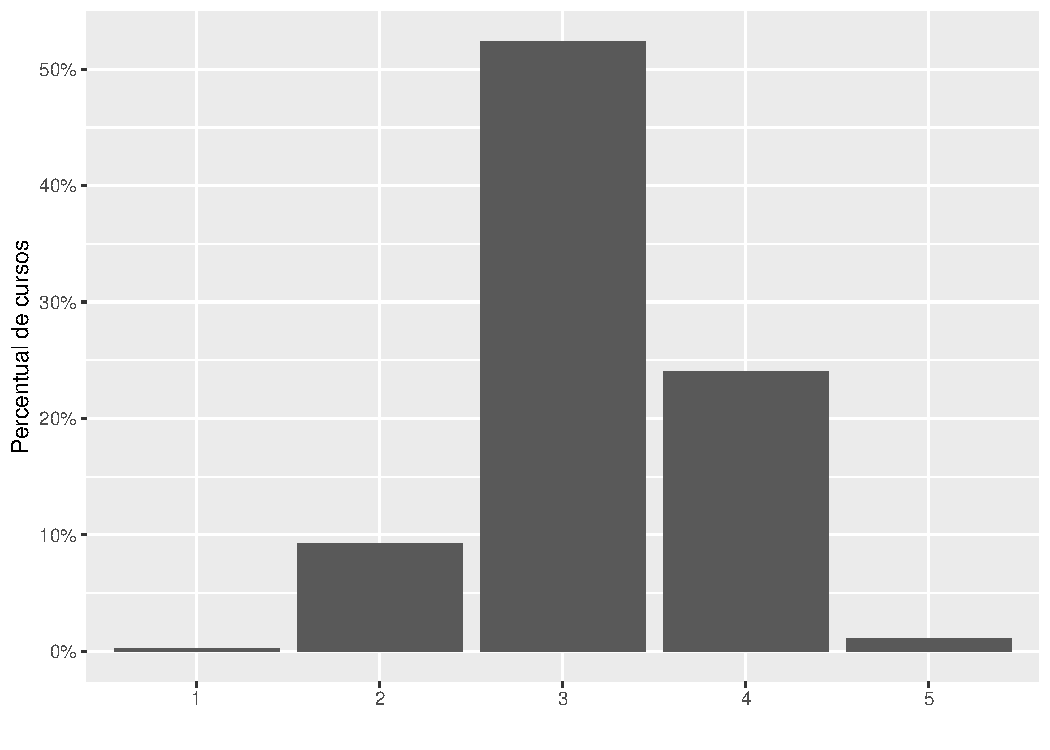
\includegraphics[scale=.3]{../graficos/latex-graph-cursos-com-conceito.pdf}
					\end{figure}
			\end{column}
			\begin{column}{0.5\textwidth}  %%<--- here
				\centering
			    % Please add the following required packages to your document preamble:
% \usepackage{booktabs}
\begin{table}[H]
\centering
\begin{tabular}{@{}lll@{}}
\toprule
\textbf{Conceito} & \textbf{Frequência} & \textbf{Percentual} \\ \midrule
1                 & 22                  & 0.3\%               \\
2                 & 753                 & 9.3\%               \\
3                 & 4252                & 52.4\%              \\
4                 & 1949                & 24.0\%              \\
5                 & 91                  & 1.1\%               \\ \bottomrule
\end{tabular}
\caption{Cursos com conceito}
\label{tbl: cursos-com-conceito}
\end{table}
			\end{column}
		\end{columns}

	\end{frame}

	\begin{frame}{Sumário estatístico das variáveis}
		% Please add the following required packages to your document preamble:
% \usepackage{booktabs}
% \usepackage{graphicx}
\begin{table}[H]
\centering
\resizebox{\textwidth}{!}{%
\begin{tabular}{@{}llllllll@{}}
\toprule
\textbf{Variável}                                         & \textbf{Média} & \textbf{Desvio padrão} & \textbf{Mediana} & \textbf{Moda} & \textbf{Mínimo} & \textbf{Máximo} & \textbf{n} \\ \midrule
Concluintes Inscritos                                     & 67.6625        & 204.194                & 39               & 25            & 1               & 11155           & 8121       \\
Concluintes Participantes                                 & 55.0494        & 162.6907               & 32               & 20            & 0               & 10059           & 8121       \\
Nota Bruta - FG                                           & 54.1955        & 6.2626                 & 53.8867          & 55.8          & 4.7127          & 80.65           & 8121       \\
Nota Bruta - CE                                           & 42.5299        & 8.228                  & 41.46            & 44.6          & 4.1746          & 80.8091         & 8121       \\
Nota Bruta - Geral                                        & 45.4587        & 7.0596                 & 44.7091          & 47.6          & 4.3141          & 79.75           & 8121       \\
Nota Contínua do Enade                                    & 2.3915         & 0.8577                 & 2.324            & 5             & 0               & 5               & 8121       \\
Nota Bruta - Organização Didático-Pedagógica              & 5.2105         & 0.481                  & 5.221            & 6             & 1.7121          & 6               & 8121       \\
Nota Padronizada - Organização Didático-Pedagógica        & 3.0204         & 1.1832                 & 3.0213           & 5             & 0               & 5               & 8121       \\
Nota Bruta - Infraestrutura e Instalações Físicas         & 4.9685         & 0.6723                 & 5.0136           & 6             & 2               & 6               & 8121       \\
Nota Padronizada - Infraestrutura e Instalações Físicas   & 3.1313         & 1.2076                 & 3.1954           & 5             & 0               & 5               & 8121       \\
Nota Bruta - Oportunidades de Ampliação da Formação       & 4.5659         & 0.8142                 & 4.5565           & 6             & 1.1905          & 6               & 8121       \\
Nota Padronizada - Oportunidades de Ampliação da Formação & 2.9541         & 1.1725                 & 2.9522           & 5             & 0               & 5               & 8121       \\
Concluintes Participantes com nota no Enem                & 28.7791        & 67.3562                & 17               & 7             & 1               & 3842            & 8121       \\
Percentual de Concluintes participantes com nota no Enem  & 0.5344         & 0.206                  & 0.5385           & 0.5           & 0.0143          & 1               & 8121       \\
Nota Bruta - IDD                                          & -0.1043        & 2.3789                 & -0.0948          & -1.5685       & -23.6519        & 24.4723         & 8121       \\
Nota Padronizada - IDD                                    & 2.4782         & 0.8428                 & 2.4758           & 0             & 0               & 5               & 8121       \\
Nr. de Docentes                                           & 26.1061        & 21.6867                & 20               & 16            & 0               & 298             & 8121       \\
Nota Bruta - Mestres                                      & 0.7633         & 0.2083                 & 0.8077           & 1             & 0               & 1               & 8121       \\
Nota Padronizada - Mestres                                & 3.5552         & 1.2234                 & 3.7796           & 5             & 0               & 5               & 8121       \\
Nota Bruta - Doutores                                     & 0.3124         & 0.2219                 & 0.2766           & 0             & 0               & 1               & 8121       \\
Nota Padronizada - Doutores                               & 1.7291         & 1.2051                 & 1.5541           & 0             & 0               & 5               & 8121       \\
Nota Bruta - Regime de Trabalho                           & 0.7592         & 0.238                  & 0.8125           & 1             & 0               & 1               & 8121       \\
Nota Padronizada - Regime de Trabalho                     & 3.6919         & 1.2766                 & 3.9688           & 5             & 0               & 5               & 8121       \\
CPC Contínuo                                              & 2.6111         & 0.5807                 & 2.609            & 1.0491        & 0.4257          & 4.6885          & 8121       \\
CPC Faixa                                                 & 3.1711         & 0.6371                 & 3                & 3             & 1               & 5               & 8121       \\ \bottomrule
\end{tabular}%
}
\caption{Sumarização da base de dados após uso do método $k$-NN: medidas estatísticas básicas}
\label{tbl: sumario-estatisico-com-knn}
\end{table}
	\end{frame}

\section{Análise do Componente Principal}

\begin{frame}{Padronização das variáveis}
	\begin{enumerate}
	%A padronização é uma etapa que precede a aplicação da ACP, porque os dados originais não estão dispostos de uma forma desproporcional.
	%O objetivo aqui é tornar a média das variáveis 0 e o desvio padrão 1.
	\item Antes da padronização:
	% Please add the following required packages to your document preamble:
% \usepackage{booktabs}
% \usepackage{graphicx}
\begin{table}[H]
\centering
\resizebox{\textwidth}{!}{%
\begin{tabular}{@{}llllllll@{}}
\toprule
\textbf{Variáveis padronizadas pelo INEP}                 & \textbf{Média} & \textbf{Desvio pradrão} & \textbf{Mediana} & \textbf{Moda} & \textbf{Mínimo} & \textbf{Máximo} & \textbf{n} \\ \midrule
Nota Padronizada - Organização Didático-Pedagógica        & 3.0202         & 1.1832                  & 3.0212           & 5             & 0               & 5               & 8121       \\
Nota Padronizada - Infraestrutura e Instalações Físicas   & 3.1312         & 1.2076                  & 3.1951           & 5             & 0               & 5               & 8121       \\
Nota Padronizada - Oportunidades de Ampliação da Formação & 2.9541         & 1.1724                  & 2.9519           & 5             & 0               & 5               & 8121       \\
Nota Padronizada - IDD                                    & 2.4801         & 0.8406                  & 2.4773           & 0             & 0               & 5               & 8121       \\
Nota Padronizada - Mestres                                & 3.5556         & 1.2232                  & 3.7834           & 5             & 0               & 5               & 8121       \\
Nota Padronizada - Doutores                               & 1.7295         & 1.2049                  & 1.5556           & 0             & 0               & 5               & 8121       \\
Nota Padronizada - Regime de Trabalho                     & 3.6922         & 1.2768                  & 3.9688           & 5             & 0               & 5               & 8121       \\ \bottomrule
\end{tabular}%
}
\caption{Estatísticas sobre as variáveis padronizadas pelo INEP}
\label{tbl: vars-padronizadas-inep}
\end{table}
	%A padronização dos dados foi feita com a utilização da função scales contida na instalação básica do R. Esta função posiciona as variáveis contı́nuas em uma unidade de escala pela subtração de sua média e divisão pelo desvio padrão (procedimento denominado z-scoring). Isso torna o desvio padrão das mesmas 1 e a média 0. Em termos matemáticos a padronização pode ser expressa pela seguinte equação:
	\item $$Z_{i}=\dfrac{X_{i}-\mu_{i}}{\sigma_{ii}}$$
	\end{enumerate}
\end{frame}

\begin{frame}{Matriz de correlação das variáveis}
	%Feita a padronização, a etapa seguinte foi ver se havia multicolinearidade entre as variáveis. Nesta matriz as variáveis são dispostas de forma que é possı́vel determinar para cada uma o seu nı́vel de correlação com os seus pares. Isso possibilita a verificação de possı́veis ocorrências de multicolinearidade.
	\begin{figure}[H]
			\centering
			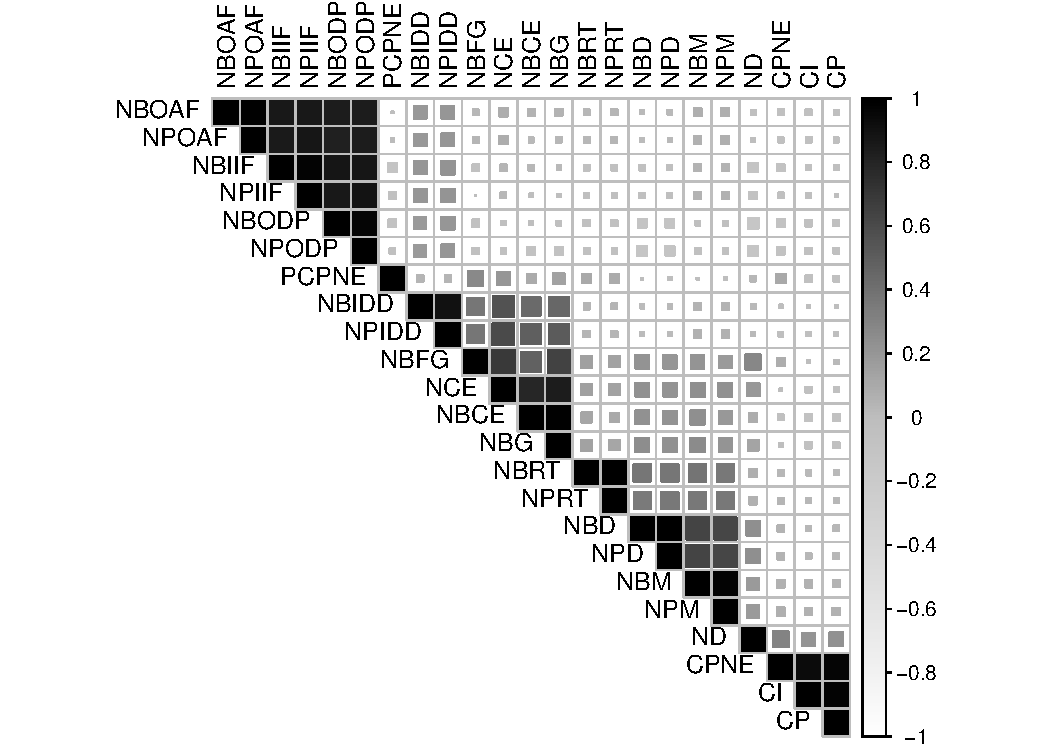
\includegraphics[scale=.5]{../graficos/latex-graph-matriz-correlacao}
			%\caption{Matriz correlograma}
			%\label{fig: matriz-correlograma1}
	\end{figure}
\end{frame}

\begin{frame}[fragile] %Aplicação da ACP: função ``principal()''
	\frametitle{Aplicação da ACP: função ``principal()''}
	%Por definição o primeiro componente é o mais representativo de todos, ou seja, é a dimensão que contabiliza a maior variabilidade possı́vel de todas as variáveis preditoras. Em outros termos é a dimensão que maximiza a variância. Com base na listagem 1, observa-se no primeiro componente (PC1) que as variáveis NBODP, NBIIF e NBOAF tem os maiores pesos. Isso significa que a organização didático pedagógica, infra-estrutura e instalações e oportunidades de ampliação da formação dos estudantes nos cursos são as variáveis mais representativas deste componente. Além disso o primeiro componente contabiliza aproximadamente 1/4 da variância de todo conjunto de componentes.

	\begin{lstlisting}[label={lst:loadings_pca}, basicstyle=\tiny]
	Loadings:
	      PC1    PC2    PC3    PC4    PC5   
	CI            0.103  0.639  0.722       
	CP            0.108  0.642  0.734       
	NBFG   0.175  0.624 -0.271  0.234       
	NBCE   0.236  0.679 -0.440  0.195       
	NBG    0.245  0.732 -0.445  0.223       
	NCE    0.285  0.725 -0.430  0.255       
	NBODP  0.891 -0.308                     
	NPODP  0.891 -0.327  0.112              
	NBIIF  0.919 -0.237  0.121              
	NPIIF  0.918 -0.237  0.145              
	NBOAF  0.918 -0.164  0.140              
	NPOAF  0.912 -0.172  0.148              
	CPNE          0.152  0.621  0.736       
	PCPNE         0.179 -0.124         0.306
	NBIDD  0.413  0.379 -0.419  0.331       
	NPIDD  0.439  0.399 -0.443  0.334       
	ND            0.343  0.232  0.208 -0.197
	NBM    0.157  0.653  0.392 -0.343 -0.242
	NPM    0.154  0.631  0.410 -0.340 -0.245
	NBD           0.670  0.376 -0.373 -0.284
	NPD           0.663  0.386 -0.373 -0.284
	NBRT          0.497  0.313 -0.334  0.712
	NPRT          0.483  0.318 -0.332  0.720
	                 PC1   PC2   PC3   PC4   PC5
	SS loadings    5.633 4.974 3.207 2.820 1.472
	Proportion Var 0.245 0.216 0.139 0.123 0.064
	Cumulative Var 0.245 0.461 0.601 0.723 0.787
	\end{lstlisting}
\end{frame}

\begin{frame}{Seleção dos componentes: \textit{``Scree plot''}}
	Tendência de horizontalização da curva de variabilidade.
	\begin{figure}[H]
			\centering
			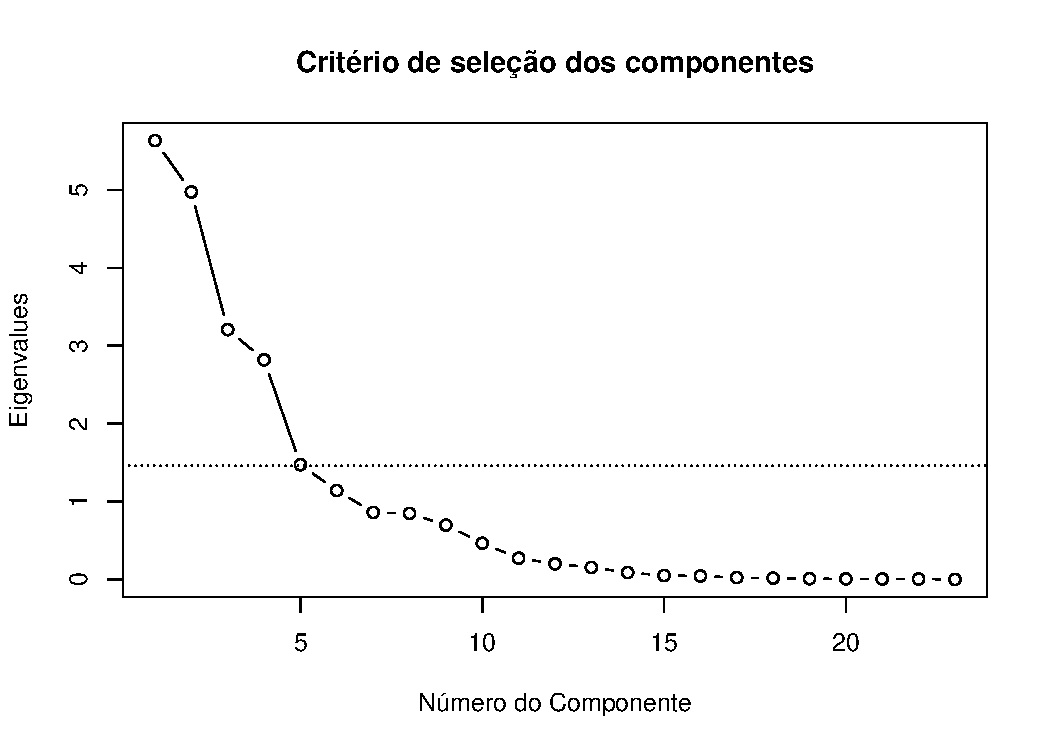
\includegraphics[scale=.50]{../graficos/latex-graph-scree-plot-pca.pdf}
			%\caption{Critério de seleção dos componentes}
			%\label{fig: scree-plot-pca}
	\end{figure}
\end{frame}

\begin{frame}{Características dos componentes}
	\begin{enumerate}
	\item PC1 (24,5\%): Organização Didático-pedagógica, Infra-estrutura e Instalações e Oportunidades de Ampliação da Formação
	\item PC2 (21,6\%): Formação Geral e Conhecimentos Específicos; Quantidade de Mestres e Quantidade de Doutores
	\item PC3 (13,9\%): Concluintes Inscritos e Percentual de Concluintes Participantes com nota no Enem
	\item PC4 (12,3\%): Apresenta o mesmo perfil de variáveis do 3º componente, contudo tem menos variabilidade
	\end{enumerate}
\end{frame}

\section{Análise do Fator}

\begin{frame}{Objetivo da aplicação}
	\begin{enumerate}
		%Neste trabalho a análise do componente principal apresentou quais variáveis são passı́veis de melhor explicarem o que influencia no desempenho de determinado curso no CPC. Foi apresentado o conjunto de variáveis e o perfil de cada componente. Contudo, é oportuno incluir mais uma camada de robustez à pesquisa pela aplicação da Análise do Fator – AF ou ( Factor Analysis – FA). Larose e Larose (2015, p. 110–111) destaca que, apesar de a ACP e AF serem técnicas de análise multivariada bem similares, a ACP deve ser em essência, um meio para a consecução da AF.
		\item Fornecer robustez aos resultados.
		%De acordo com Hair et al. (1998, p. 93) a AF desempenha um papel importante na identificação das interações entre as variáveis por intermédio do agrupamento (em fatores) das mesmas de acordo com seu grau de relação. Esse procedimento permite a redução da dimensionalidade. Isso quer dizer que procura-se descrever um evento utilizando um conjunto menor de variáveis relativamente ao conjunto original estudado com o mı́nimo de perda de informação.
		\item Redução de dimensionalidade
	\end{enumerate}
\end{frame}

\begin{frame}{Características dos fatores}
	\begin{enumerate}
	\item PA1 (22,7\%): Organização Didático-pedagógica, Infra-estrutura e Instalações e Oportunidades de Ampliação da Formação
	\item PA2 (20,2\%): Formação Geral e Conhecimentos Específicos; Quantidade de Mestres e Quantidade de Doutores
	\item PA3 (12,1\%): Concluintes Inscritos, Concluintes Participantes e Concluintes Participantes com Nota no Enem
	\item PA4 (10,3\%): Concluintes Inscritos, Concluintes Participantes e Concluintes Participantes com Nota no Enem e nota no Indicador de Diferença de Desempenho
	\end{enumerate}
\end{frame}

\section*{}
\begin{frame}{Resultados}
	\begin{enumerate}
	%acúmulo de 1/4 da variabilidade no primeiro componente indica que: 
	\item A percepção dos alunos tem papel decisivo na composição do CPC
	%Em relação à primeira variável, é possı́vel afirmar que fatores como coerência da estrutura curricular com os objetivos dos cursos; adequação e atualização das ementas e das disciplinas; uma seleção de conteúdos satisfatória; adequação, atualização e relevância da bibliografia; dentre outros, podem ser favoráveis à melhora do indicador de qualidade do curso de graduação.
	\item Estrutura curricular alinhada aos objetivos do curso
	%ambientes projetados para atender a todos os requisitos necessários para a realização das atividades de ensino; que levem em consideração o conforto não apenas dos discentes, mas de toda comunidade acadêmica e que sejam adequados para questões relacionadas à acessibilidade. Aliado a estes, sistema de segurança, iluminação, ventilação, equipamentos e mobiliários adequados, podem impactar de forma significativa o CPC.
	\item Ambientes de ensino e espaço de convivência adequados.
	%Finalmente, as Oportunidades de Ampliação da Formação tem grande importância na composição do CPC. Devem ser criados meios para que, durante o perı́odo da graduação, sejam apresentadas aos alunos as alternativas de prosseguimento dos estudos. Arrisca-se afirmar que isso proporciona resultados não apenas no que se refere ao indicador de qualidade do curso superior, mas também implica em avanços em termos de ampliação da fronteira do conhecimento.
	\item Oportunidades de Ampliação da formação
	\end{enumerate}
\end{frame}

\begin{frame}{Conclusão}
	\begin{enumerate}
	%Apesar de a educação ser um fator essencial para o desenvolvimento de uma nação, o Brasil ainda desponta como uma das nações com maior proporção de adultos que não tiveram aeducação primária (OCDE, 2017, p. 44). Por esse motivo, acredita-se que as contribuições ao tema, por menores que sejam, são valiosas. Ainda que se reconheça a relevância das fases de base da educação, bem como a variedade de instrumentos de avaliação das mesmas, buscou-se neste trabalho analisar a sistemática de avaliação do ensino superior.
	\item Relevância da educação na vida do indivíduo e importância para o desenvolvimento de uma nação
	%Procurou-se, fornecer um instrumento informativo, quiça fundamentador de tomada de decisão aos atores responsáveis, direta e indiretamente pela gestão das unidades de ensino superior e cursos de graduação. À comunidade acadêmica das IES, foram apresentados os principais elementos que devem ser estimulados, desenvolvidos, e mantidos de forma a lograr qualidade na avaliação do Enade.

	%Aos desenvolvedores de polı́ticas educacionais, busca-se por meio desta pesquisa viabilizar conteúdo informacional para que promova-se a adequada expansão do ensino superior às diversas classes da sociedade, sem negligenciar a qualidade do mesmo.
	\item Expansão consciente do ensino no país
	\end{enumerate}
\end{frame}



\end{document}